
\chapter{Esittely}

\section{Arduino}

”Open Source Electronics Prototyping Platform”

Arduino/Genuino on avoimeen laitteistoon ja ohjelmistoon perustuva mikrokontrolleri-elektroniikka-alusta ja ohjelmointiympäristö. Arduinon avulla toteutetussa laitteessa on kaksi kokonaisuutta: Arduinoon liitetty ulkoinen kytkentä ja Arduinoon syötetty ohjelma.

Arduinokortin INPUT-napoihin voi liittää erilaisia antureita, säätimiä tai kytkimiä, jotka ohjaavat OUTPUT- napoihin kytkettyjä ledejä, releitä, servoja tai moottoreita. Laitteen toiminnot määritetään laitteeseen syötetyllä ohjelmalla. Arduino-ympäristö tarjoaa helpon ja halvan keinon opetella elektroniikkaa ja ohjelmointia nykyaikaisella tavalla.

Arduino on hyvin avoin konsepti ja erilaisia *duino-tuotteita myydään nettikauppojen välityksellä huokeaan hintaan. Euroopassa ”aidot” Arduino-tuotteet myydään Genuino-nimen alla. Projektin kotisivu on osoitteessa www.arduino.cc.


\newpage
\subsection*{Arduinon osat}

\begin{figure}[h!]
    \begin{tikzpicture}[remember picture]
\node (fig1) at (0,0)
       {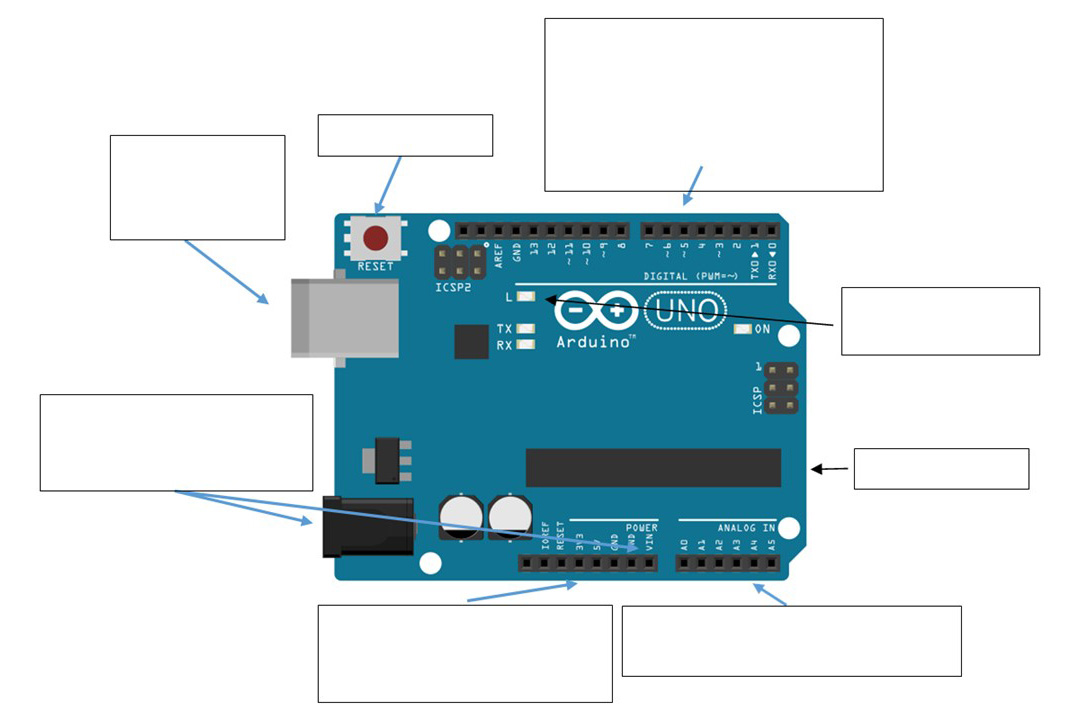
\includegraphics[scale=0.55]{kuvat/arduino.jpg}};
\end{tikzpicture}
\begin{tikzpicture}[remember picture, overlay]
       \node [align=left,] at (10.5,9.55) {\small 14 digitaalista kytkentäpinniä\\\small (voidaan ohjelmallisesti määrittää\\\small  joko INPUT-tai OUTPUT-pinneiksi)\\\small LOW = 0 = 0 V \\\small  HIGH = 1 = +5 V };
      \node [align=left] at (2.6,4.65) {\small Ulkoinen virransyöttö\\\small (6...15 V, 2,1 mm virtaliitin\\\small tai Vin -pinni)};
      \node [align=left] at (3,8.4) {USB-liitin\\ koodin \\ja virran
    syöttö };
      \node [align=left] at (5.95,9.15) {Reset-nappula};
      \node [align=left] at (13.8,6.45) {Pinniin 13 kytketty\\ledi};
      \node [align=left] at (13.8,4.3) {Mikrokontrolleri};
      \node [align=left] at (6.9,1.6) {\small Virtaliitäntä kytkentöjä varten,\\\small 5 V, GND (0 V eli maa)};
      \node [align=left] at (11.65,1.75) {\small 6 analogista kytkentäpinniä A0-A5\\\small lukevat jännitettä 0--5 V};
      

\end{tikzpicture}
    \caption{Arduino Unon osat}
    \label{fig:arduino_uno}
\end{figure}

%Arduinon osat ja niiden kuvaustekstit


\newpage
\subsection*{Koekytkentälevy}
Koekytkentälevy Kuva:\ref{fig:koekytkentalevy} (engl. Breadboard) on alusta, jolle voi koota kytkennän tarvitsematta juottaa komponentteja kiinni. Laitteet toteutetaan sijoittamalla komponentit koekytkentälevylle, jolloin samassa rivissä olevat komponenttien pinnit ovat yhteydessä toisiinsa. Ulkoiset liitokset Arduinoon ja muihin komponentteihin tehdään hyppylangoilla

Arduino/Genuino Starter Kit on aloittelevalle harrastajalle sopiva sarja, jossa Arduinokortin, komponenttien ja kattavan ohjekirjan lisäksi saa rakentelualustan, jossa samalle alustalle on asennettu Arduino Uno ja koekytkentälevy. Hieman halvemmalla alkuun pääsee hankkimalla pelkän Arduinokortin ja koekytkentälevyn. Tällöin muut komponentit täytyy kuitenkin hankkia erikseen.

Tutkimustöiden kytkentäkuvat on piirretty toteutettavaksi Starter Kitillä.



%koekytkentälevy
\begin{figure}[h!]
    \centering
    \begin{tikzpicture}[remember picture]
\node (fig1) at (0,0)
       {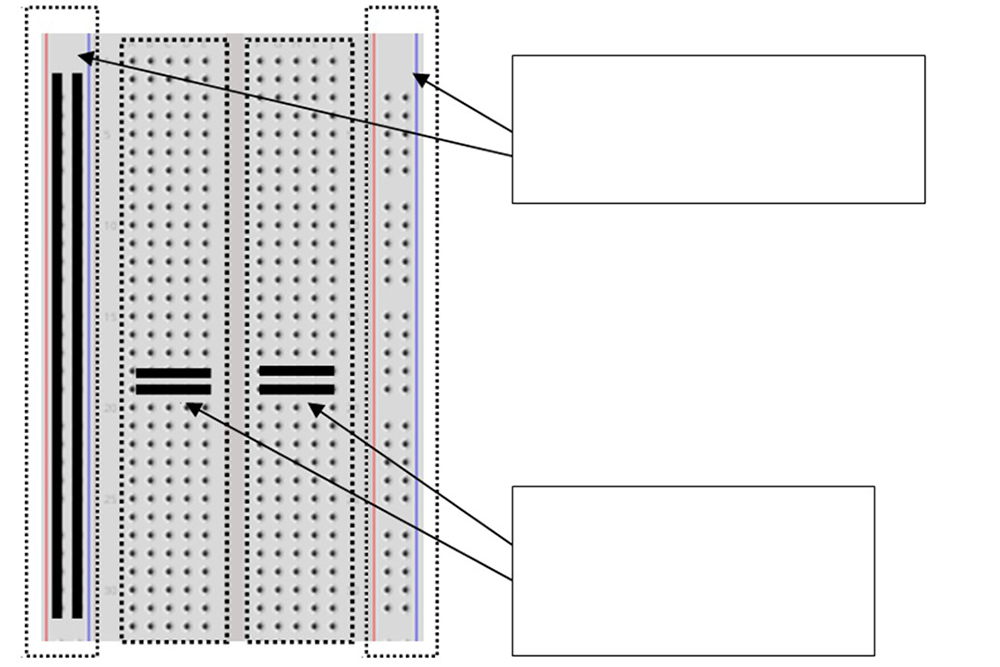
\includegraphics[scale=0.40]{kuvat/koekytkentalevy.jpg}};
\end{tikzpicture}
\begin{tikzpicture}[remember picture, overlay]
       \node [align=left,] at (-4.5,1.5) {Vaakarivi samaa\\ johdinta. Ura katkaisee johtimen.\\ Tähän kohtaan\\varsinainen kytkentä};
       \node [align=left,] at (-4.6,7.7) {Pystyrivi samaa johdinta.\\Tähän kytketään yleensä\\virransyöttö +5 V tai 0 v (GND) };
\end{tikzpicture}
    \caption{Koekytkentälevy, rivit ja sarakkeet levyllä. }
    \label{fig:koekytkentalevy}
\end{figure}
\newpage

\subsection*{Ohjelmointiympäristöt}

Lataa Arduinon ohjelmointiympäristö osoitteesta https://www.arduino.cc/en/Main/Software. Ohjelma on ilmainen ja voit valita nappulan ”Just download”. Jos haluat tukea ohjelman kehittäjiä, niin voit valita summan ja nappulan ”Contribute \& Download”. Sivulta löytyy Windows-, Mac- ja Linux-versiot.

Windows-versiota asennettaessa asennusohjelma antaa mahdollisuuden asentaa automaattisesti myös USB-ajurin. Ajuri kannattaa asentaa, koska ilman sitä tietokone ei tunnista Arduinokorttia.



\begin{center}
\begin{fminipage}{10cm}
\textbf{Ohjelman käyttö:}
\begin{enumerate}
    \item Avaa Arduino-ohjelma koneelle 
    \item Kytke Arduino-kortti USB-johdolla koneelle
    \item Tarkista Tools/Työkalut-valikosta Board/Kortti (Arduino Uno) ja Serial Port/Portti (yleensä COM3 tai suurempi)
    \item Ohjelma ”Sketch” ladataan Arduinolle vasemman yläkulman nuolella merkitystä nappulasta

\end{enumerate}
\end{fminipage}
\end{center}

Seikkaperäiset ohjeet ovat sivulla https://www.arduino.cc/en/Guide/Windows. Ohjeet löytyvät myös editoriohjelman Apua-toiminnosta.
\begin{center}
\begin{fminipage}{10cm}
    Ohjelmoinnin tärkein apusivusto on Arduinon oma opas osoitteessa https://www.arduino.cc/en/Reference/HomePage.
\end{fminipage}
\end{center}


\begin{figure}[h!]
    \centering
        \begin{tikzpicture}[remember picture]
\node (fig1) at (0,0)
       {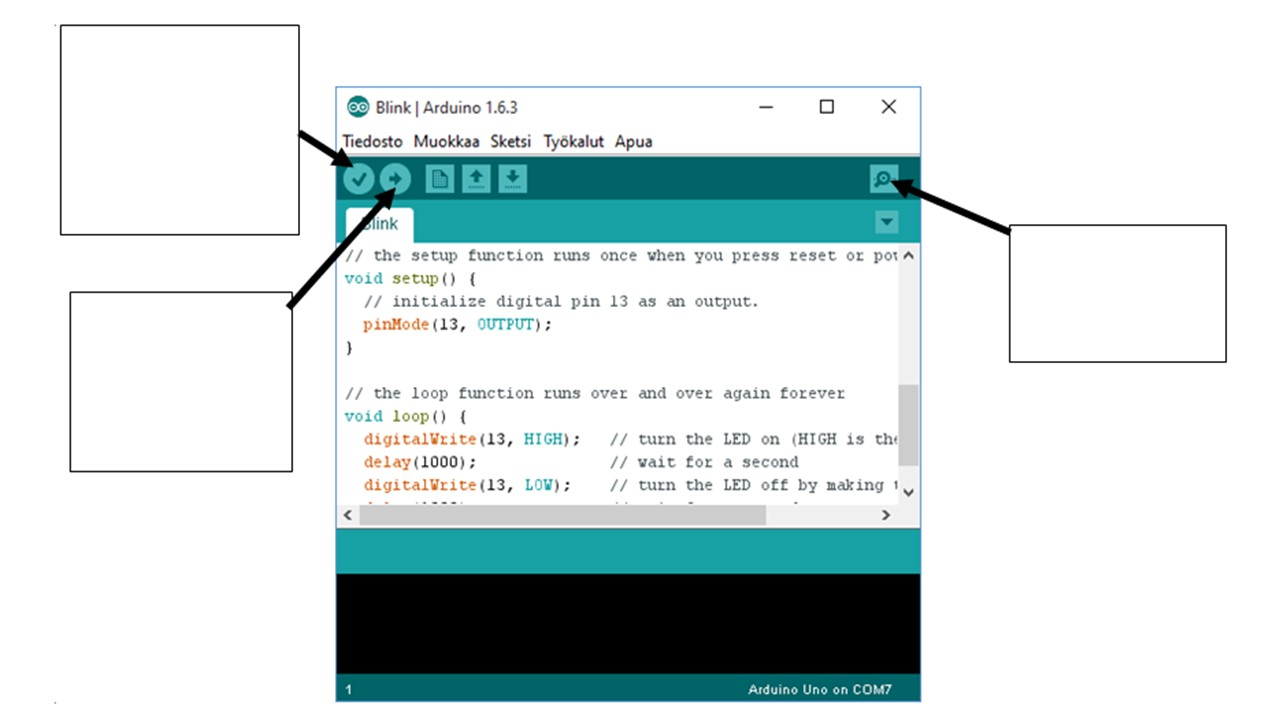
\includegraphics[scale=0.45]{kuvat/ohjelmointiymparisto.jpg}};
\end{tikzpicture}
\begin{tikzpicture}[remember picture, overlay]
       \node [align=left,] at (-5.4,7.7) {\textit{Verify/Tarkista}\\Ohjelma\\tarkistaa\\mutta ei ladata\\Arduinolle };
       \node [align=left,] at (-5.4,4.7) {\textit{Upload/Lataa}\\Ohjelma\\ladataan\\Arduinolle };
       \node [align=left,] at (5.85,5.7) {Avaa sarjaportin\\monitorointi-\\ikkunaan };
\end{tikzpicture}
    \caption{Arduinon ohjelmointiympäristö ja keskeiset hallinnointi painikkeet. }
    \label{fig:ohjelmointiymparisto}
\end{figure}

% \begin{figure}[h!]
%     %\centering
%     \begin{tikzpicture}[remember picture]
%     \node at (0,0) {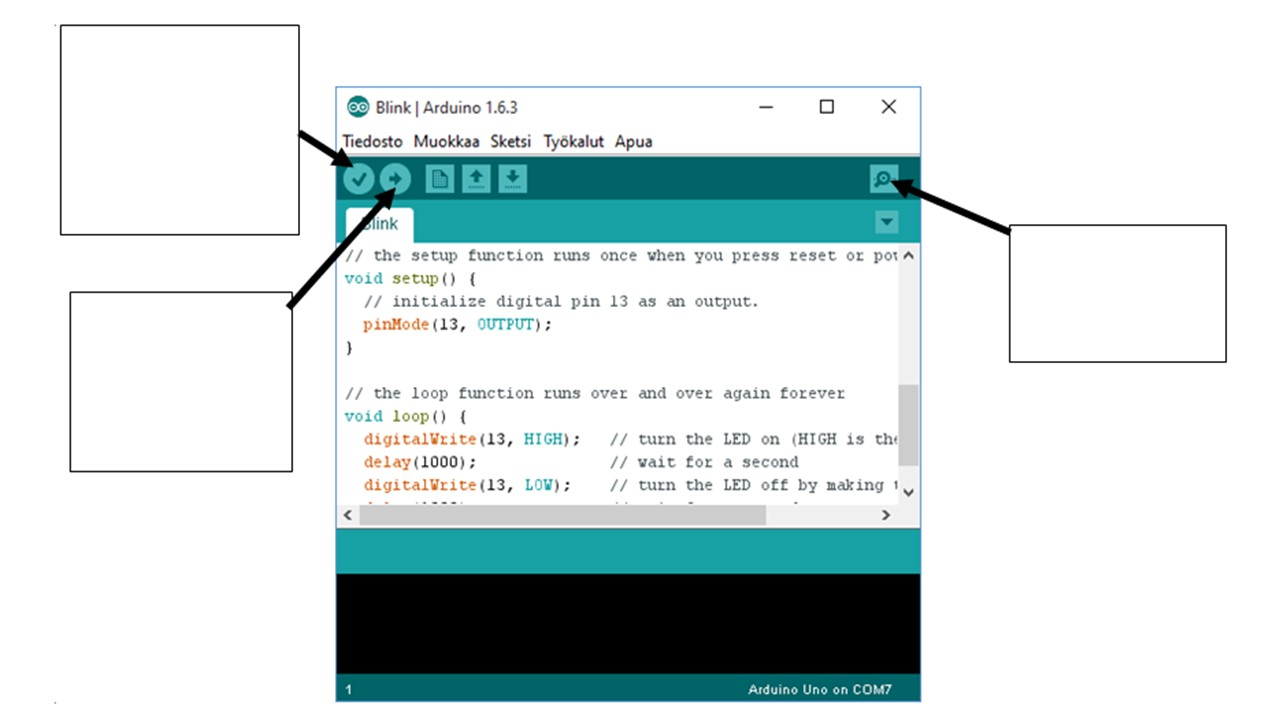
\includegraphics[scale=0.4]{kuvat/ohjelmointiymparisto.jpg}};
%     \end{tikzpicture}
%     \begin{tikzpicture}[overlay,remember picture]
    
%     \end{tikzpicture}
%     \caption{Arduinon ohjelmointiympäristö ja keskeiset hallinnointi painikkeet. }
%     \label{fig:ohjelmointiymparisto}
% \end{figure}